\chapter{Error Prediction Methods and Transfer Function Models}
\label{chap:error-prediction-methods-tf}

We assume that the complete system model is given by
\begin{equation}
  \label{eq:PEM-tf-models}
  y(k) = G(z)u(k) + H(z)e(k).
\end{equation}
Prediction error-based identification methods estimate the transfer functions $G(z)$ and $H(z)$, parametrised as $G(z,\theta)$ and $H(z,\theta)$, by minimizing the objective function $J(\epsilon)$, a function of the prediction error $\epsilon(k,\theta)$
\begin{equation*}
  \epsilon(k,\theta) \doteq y(k) - \hat{y}(k,\theta).
\end{equation*}
The prediction $\hat{y}(k,\theta)$ for the time $k$ is a function of the previous measurements and inputs at $k-1,\ k-2,\ldots$ only.

%%%%%%%%%%%%%%%%%%%%%%%%%%%%%%%%%%%%%%%%%%%%%%%%%%%%%%%%%%%%
\section{Prediction}
\label{sec:prediction}

We assume that $H(z)$ is monic\footnote{Monic means that $h(0)=1$:
\begin{equation*}
  H(z) = 1 + \sum_{k=1}^\infty h(k)z^{-k}.
\end{equation*}} and stable\footnote{$H(z)$ has only poles strictly inside the unit circle.}. In this case, given the filtered noise $v(k)=H(z)e(k)$, $e(k)$ can be reconstructed from $v(k)$ as
\begin{equation}
  \label{eq:noise-reconstruction}
  e(k) = H^{-1}(z)v(k).
\end{equation}

We now seek to predict $v(k)$ given the past values up to time $k-1$: this is called the \emph{one-step ahead} estimate. Since $H(z)$ is monic, we split the filtered noise contribution into the term $e(k)$ and other terms up to time $k-1$
\begin{equation}
  \label{eq:prediction-split-filtered-noise}
  v(k) = H(z)e(k) = e(k) + \left(H(z)-1\right)e(k)
\end{equation}
The \emph{predicted} filtered noise $\hat{v}(k|k-1)$ is
\begin{equation*}
  \hat{v}(k|k-1) = (H(z)-1)e(k).
\end{equation*}
This can be intuitively understood because the error probability function distribution for $\{e\}$ has zero mean\footnote{Had the probability distribution $f_e(x)$ not had a zero mean, we would have to modify the predition according to
  \begin{equation*}
    \hat{v}(k|k-1) = \arg\max_x f_e(x - m(k-1)),\hspace{2em} m(k-1) = (H(q)-1)e(k).
  \end{equation*}}: if we were left to guess $e(k)$, we would guess $e(k)=0$. Making use of eq.~\eqref{eq:noise-reconstruction}, the one-step ahead estimate
\begin{equation}
  \label{eq:filtered-noise-one-step-prediction}
  \hat{v}(k|k-1) = \left(1-H^{-1}(z)\right)v(k)
\end{equation}
is determined only from the knowledge of the past values of $v$ up to $k-1$.

For the model of eq.~\eqref{eq:PEM-tf-models}, the one-step ahead predictor
\begin{equation}
  \label{eq:one-step-ahead-predictor-noise}
  \hat{y}(k|k-1) = G(z)u(k) + \hat{v}(k|k-1)
\end{equation}
can be rewritten with the help of the expression for $\hat{v}(k|k-1)$ as\footnote{Using $v(k) = y(k) - G(z)u(k)$
  \begin{equation*}
    \hat{y}(k|k-1) = G(z)u(k) + \left(1-H^{-1}(z)\right)\left(y(k) - G(z)u(k)\right).
  \end{equation*}
Note that $y_0(k)=G(z)u(k)$ is the evolution of the noiseless true system, so that eq.~\eqref{eq:one-step-ahead-predictor-noise} could also be written as $\hat{y}(k|k-1) = y_0(k) + \hat{v}(k|k-1)$. However we seek an expression that involves the measured outputs $y(k)$ and expressing the one-step head predictor as a function of the unknown true system is of no use to us.\label{fn:noiseless-regressor}}
\begin{equation}
  \label{eq:one-step-ahead-predictor}
  \hat{y}(k|k-1) = H^{-1}(z)G(z)u(k) + \left(1-H^{-1}(z)\right) y(k).
\end{equation}
The prediction error\footnote{Although in class the algebra was worked out, that $\epsilon(k|k-1)=e(k)$ is no surprise: $e(k)$ was the term that was discarded from $v(k)$ to compute the predicted filtered noise $\hat{v}(k|k-1)$.}
\begin{equation}
  \label{eq:one-step-ahead-predictor-error}
  \epsilon(k,|k-1) = y(k) - \hat{y}(k|k-1) = e(k)
\end{equation}
is the noise $e(k)$: the \emph{innovation} is the part of the output prediction that cannot be estimated from past measurements.

%%%%%%%%%%%%%%%%%%%%%%%%%%%%%%%%%%%%%%%%%%%%%%%%%%%%%%%%%%%%
\subsection{Example: Moving Average}

The model
\begin{equation*}
  v(k) = e(k) + ce(k-1) \rightarrow H(z) = 1+cz^{-1}
\end{equation*}
is invertible when $|c|<1$. The one-step ahead predictor eq.~\eqref{eq:filtered-noise-one-step-prediction} can be expressed in terms of the error $e(k-1)$ using eq.~\eqref{eq:one-step-ahead-predictor-error}
\begin{equation*}
  \hat{v}(k|k-1) = \left(1-H^{-1}(z)\right)H(z)e(k) = cz^{-1}e(k) =  ce(k-1)
\end{equation*}

%%%%%%%%%%%%%%%%%%%%%%%%%%%%%%%%%%%%%%%%%%%%%%%%%%%%%%%%%%%%
\section{Family of Transfer-Function Models}
\label{sec:family-tf-models}

The advantage of the transfer-function models is that they can be described by fewer parameters and that the inputs required to identify the system do not have to be persistently exciting as it is the case when one wants to identify frequency or time-response: we have seen in Sect.~\ref{} that for frequency domain methods, the order of excitation must be double the number of complex estimates of the transfer function $G(e^{j\omega_n})$ since gain and phase must be determined for each frequency; for a time response one requires the same persistency order as the number of impulse response terms.

If we control the input, this requirement is easy to satisfy. If on the other hand the data is given, this may not be the case and in these situations, one is better off looking for transfer functions/state space representations because of the reduced numbers of parameters to identify.

Prediction error-based identification methods construct the prediction error\footnote{Here we are seeking the unknown parameters $\theta$ for a known model for which we can construct the one-step ahead predictor $\hat{y}(k,\theta)$, parametrized by $\theta$. Since $\theta$ is unknown, we cannot say just yet that $\epsilon(k,\theta) = e(k)$.

  I also do not know if $\min_\theta ||\epsilon(\theta)||_2^2 = \sum_k ||e(k)||_2^2$ but I suspect this is the case when $e(k)$ is Gaussian-distributed.}
\begin{equation}
  \label{eq:prediction-error-parametrized}
  \epsilon(k,\theta) = y(k) - \hat{y}(k,\theta)
\end{equation}
from the (one-step ahead) predictor $\hat{y}(k,\theta)$ which is based on the guesses $\hat{G}(z)=G(z,\theta)$ and $\hat{H}^{-1}(z)=H^{-1}(z,\theta)$, the guesses being parametrized by $\theta$. The optimal $\theta^\star$ is the argument that minimizes the cost function $J=J(\epsilon)$
\begin{equation*}
  \theta^\star = \arg \min_\theta J(\epsilon(k,\theta)).
\end{equation*}
Typical choices for the objective functions $J(\epsilon)$ are the 2-norm $||\epsilon||_2^2$ or the maximum deviation, the $\infty$-norm $||\epsilon||_\infty$. The kind of minimization depends on how the models $G(q)$ and $H^{-1}(q)$ are parametrised: in general, the parametrization will not be linear and the optimization may not be convex. Note moreover that the minimization of $||\epsilon||_2^2$ is not equivalent to the least squres method, unless  $H(z)=1$:
\begin{equation*}
  y(k) = G(z)u(k) + e(k).
\end{equation*}

Since this approach does not require an a-priori knowlege of the system, it is also called the \emph{black-box} approach.

%%%%%%%%%%%%%%%%%%%%%%%%%%%%%%%%%%%%%%%%%%%%%%%%%%%%%%%%%%%%
\subsection{Equation Error Model Structure (ARX)}
\label{sec:ARX}

%The numerator is the moving average (MA) part, the denominator the autoregressive (AR) part, X for the exogeraneous (external) input.

The ARX model
\begin{equation}
  \label{eq:ARX-model}
  y(k) = B(z)u(k) + \left(1-A(z)\right)y(k) + e(k)
\end{equation}
is a simple input-output relationship where the error enters as a direct term: this model covers a limited set of real-world problems, for instance those where the perturbation act as a force. We take
\begin{equation*}
  A(z) = 1 + a_1z^{-1} + \ldots + a_nz^{-n},\hspace{2em} B(z) = b_1z^{-1} + \ldots + b_mz^{-m}
\end{equation*}
where $A(z)$ is monic and $B(z)$ does not contain a constant term, \textit{i.e.} the model has no feed-through. It corresponds to the model of eq.~\eqref{eq:PEM-tf-models} with
\begin{equation*}
  G(z) = \frac{B(z)}{A(z)},\hspace{2em}H(z) = \frac{1}{A(z)}.
\end{equation*}
and generates the one-step ahead predictor
\begin{equation}
  \label{eq:one-step-ahead-ARX}
  \hat{y}(k|k-1) = \left(1-A(z)\right)y(k) + B(z)u(k)
\end{equation}
either by plugging $G(z)$ and $H^{-1}(z)$ in eq.~\eqref{eq:one-step-ahead-predictor} or by using the result of eq.~\eqref{eq:one-step-ahead-predictor-error} in eq.~\eqref{eq:ARX-model}.

We now seek the estimates $\hat{B}(z,\theta)$ and $\hat{A}(z,\theta)$ parametrized by the \emph{parameter vector} $\theta$ which contains the unknown coefficients of the polynomials $A(z)$ and $B(z)$
\begin{equation*}
  \theta =
  \begin{bmatrix}
    a_1 & \ldots & a_n & b_1 & \ldots & b_m
  \end{bmatrix}^\top
\end{equation*}
This generates the one-step ahead predictor
\begin{equation*}
  \hat{y}(k,\theta) = \left(1-\hat{A}(z,\theta)\right)y(k) + \hat{B}(z)u(k).
\end{equation*}
that can be written in linear form
\begin{equation*}
  \varphi^\top(k) =
  \begin{bmatrix}
    -y(k-1) & \ldots & -y(k-n) & u(k-1) & \ldots & u(k-m)
  \end{bmatrix}.
\end{equation*}
using the \emph{regressor vector} $\varphi(k)$ that contains the outputs and inputs.

$\theta$ is found by minimization of the prediction error $\epsilon(k,\theta) = y(k) - \hat{y}(k,\theta)$: when $\theta$ is the true parameter vector $\theta_0$, then $\epsilon(k,\theta_0)=e(k)$. Generally, one minimizes the 2--norm $||\epsilon(k,\theta)||_2^2$: this  is solved in MATLAB by
\begin{equation}
  \label{eq:ARX-solution}
  %\Phi\hat{\theta} = Y\rightarrow
  \hat{\theta} = \Phi \backslash Y,\hspace{2em} \Phi \doteq
  \begin{bmatrix}
    \varphi^\top(1) \\ \varphi^\top(2) \\ \ldots \\ \varphi^\top(N)
  \end{bmatrix}, \hspace{1em} Y \doteq
  \begin{bmatrix}
    y(1) \\ y(2) \\ \ldots \\ y(N)
  \end{bmatrix}
\end{equation}
The first element of the regressor is $\varphi(1)$ that depends on the past indeces up to $k=0$: these are the initial conditions. They are usually specified by the system being at rest; otherwise, one must drop a certain amount of entries (how many exactly?)

%%%%%%%%%%%%%%%%%%%%%%%%%%%%%%%%%%%%%%%%%%%%%%%%%%%%%%%%%%%%
\subsection{ARX: Estimate Bias}
\label{sec:estimate-bias-ARX}

The numerical example in class (slides 9-30 to 9--34) confused me. In the first situation we have
\begin{equation*}
  \frac{B(z)}{A(z)} = \frac{bz^{-1}}{1 + az^{-1}}, \hspace{2em} H(z)=1.
\end{equation*}
The one-step ahead predictor is
\begin{equation*}
  \hat{y}(k|k-1) = y(k) - e(k) = \frac{B(z)}{A(z)}u(k) = \varphi_0^\top(k)\theta_0
\end{equation*}
is nothing else than the evolution of the true system. The regressor $\Phi_0$ must be constructed from the true $y_0(k) = \frac{B(z)}{A(z)}u(k)$: using instead the measured $y(k)$ gives the bias of slide 9--30. (See also discussion in Sect.~\ref{sec:estimation-bias}.)

\begin{figure}[h]
  \centering
  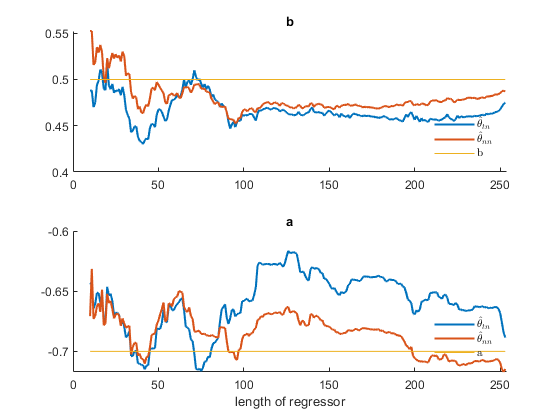
\includegraphics[width=0.8\textwidth]{09_lect/ARX-bias.png}
  \caption{Comparison of estimates with true and noisy regressors and data for a PRBS input signal with $O=7$ and $N=127$. The estimates start from a minimum regressor length of $10$. The code is in \texttt{09\_lect/SysID\_ARX.m}.}
  \label{fig:estimate-bias-ARX}
\end{figure}

In the second situation, we take the noise to be $H(z) = \frac{1}{A(z)}$. In Fig.~\ref{fig:estimate-bias-ARX} I compare the solutions of the least square problems
\begin{equation*}
  \hat{\theta}_{tn} \doteq \Phi_0\backslash Y,\hspace{2em} \hat{\theta}_{nn} \doteq \Phi\backslash Y
\end{equation*}
as a function of the number of elements in the regressor, just as it was done in class for the first problem. Only by looking at the graph, it is not possible to tell whether an estimate is biased, but repeating the experiment reveals that neither $\hat{\theta}_{nn}$ (as expected) nor $\hat{\theta}_{tn}$ (perhaps unexpectedly) are biased.

The explanation is the following: the (noisy) system's evolution is
\begin{equation*}
  y(k) = (1-A(z))y(k) + B(z)u(k) + e(k) = \varphi^\top(k)\theta_0 + e(k)
\end{equation*}
and I \emph{pick}\footnote{The word ``pick'' is emphasized: it is the true predictor but, at least for ARX, it seems to me that the most convenient predictor for the solution of the least-squares is whatever regressor the true system uses.} the one-step ahead predictor to be $\hat{y}(k,\theta) = \varphi^\top(k)\theta$. Their difference
\begin{equation*}
  y(k)-\hat{y}(k,\theta) = \varphi^\top(k)(\theta_0-\theta) + e(k)
\end{equation*}
is minimized when $\theta=\theta_0$ since $e(k)$ is Gaussian distributed: this is the case $\Phi\backslash Y$. On the other hand, we can also write
\begin{equation*}
  y(k) = y_0(k) + \frac{1}{A(z)}e(k) = \varphi_0^\top(k)\theta_0 + \frac{1}{A(z)}e(k)
\end{equation*}
and I \emph{choose}\footnote{ As mentioned already in footnote~\ref{fn:noiseless-regressor}, the noiseless regressor $\Phi_0$ cannot be constructed from the noisy data unless (I think) $H(z)=1$ when $\hat{y}(k|k-1)=y_0(k)$.} the predictor to be $\hat{y}(k,\theta) = \varphi_0^\top(k)\theta$. Their difference
\begin{equation*}
  y(k) - \varphi_0^\top(k)\theta = \varphi_0^\top(k)(\theta_0-\theta) + \frac{1}{A(z)}e(k)
\end{equation*}
is also minimized when $\theta=\theta_0$ since $\frac{1}{A(z)}e(k)$ has Gaussian distribution (although it is now correlated). This means
\begin{equation*}
  \EE{\Phi\backslash Y} = \EE{\Phi_0\backslash Y} = \theta_0
\end{equation*}
are both unbiased.

%%%%%%%%%%%%%%%%%%%%%%%%%%%%%%%%%%%%%%%%%%%%%%%%%%%%%%%%%%%%
\subsection{ARMAX Model Structure}
\label{sec:ARMAX}

The ARX model structure is not very flexible with regards to the noise model requiring it to have the particular structure $\frac{1}{A(z)}$. The ARMAX transfer function model partially relaxes this: it has the form
\begin{equation}
  \label{eq:ARMAX-model}
  A(z)y(k) = B(z)u(k) + C(z)e(k)
\end{equation}
where $A(z)$ and $B(z)$ are as in ARX and $C(z)$ is monic. It corresponds to the model of eq.~\eqref{eq:PEM-tf-models} with
\begin{equation*}
  G(z) = \frac{B(z)}{A(z)},\hspace{2em} H(z) = \frac{C(z)}{A(z)}
\end{equation*}
and with the one-step ahead predictor\footnote{In alternative to plugging the expressions for $G(z)$ and $H^{-1}(z)$ into eq.~\eqref{eq:one-step-ahead-predictor}, the one-step ahead predictor can be equally easily obtained from eq.~\eqref{eq:ARMAX-model} and eq.~\eqref{eq:one-step-ahead-predictor-error}:
  \begin{align*}
    \hat{y}(k|k-1) &= y(k) - e(k) \\
                   &=\left(1-A(z)\right)y(k) + B(z)u(k) + \left(C(z)-1\right)e(k) \\
                   &= \left(1-A(z)\right)y(k) + B(z)u(k) + \left(C(z)-1\right)\left(y(k)-\hat{y}(k|k-1)\right).
  \end{align*}
  This operation only makes sense when $H(z)$ is stably invertible though: at least $C(z)$ cannot have unstable zeros.

  Consistency check: this expression reduces to ARX one-step ahead predictor eq.~\eqref{eq:one-step-ahead-ARX} when $C(z)=1$.}
\begin{equation}
  \label{eq:one-step-ahead-ARMAX}
  \hat{y}(k|k-1) = (1-A(z))y(k) + B(z)u(k) + (C(z)-1)\left(y(k)-\hat{y}(k|k-1)\right)
\end{equation}

Introducing the regression vector
\begin{equation*}
  \varphi^\top(k,\theta) =
  \begin{bmatrix}
    -y(k-1) & \ldots & u(k-1) & \ldots & \epsilon(k-1,\theta) & \ldots
  \end{bmatrix}
\end{equation*}
eq.~\eqref{eq:one-step-ahead-ARMAX} induces the pseudolinear regression
\begin{equation}
  \label{eq:pseudolinear-regression-ARMAX}
  \hat{y}(k,\theta) = \varphi^\top(k,\theta) \theta
\end{equation}
the equation is non-linear because the unknown appears also in the regressor $\varphi^\top(k,\theta)$.

Since the regressor is pseudolinear, using non-linear least-squares to estimate $\theta$ will result in a biased estimate (why exactly?).

%%%%%%%%%%%%%%%%%%%%%%%%%%%%%%%%%%%%%%%%%%%%%%%%%%%%%%%%%%%%
\subsection{Constrained Minimization}
\label{sec:ARMAX-minimization}

Using eq.~\eqref{eq:pseudolinear-regression-ARMAX} and eq.~\eqref{eq:prediction-error-parametrized}, we have that $y(k) = \varphi^\top(k,\theta) \theta + \epsilon(k,\theta)$: this is used as the constraint in the optimization-based algorithm for the solution to the ARMAX problem:
\begin{equation*}
  \begin{aligned}
    \min_{\theta,\epsilon}\ & ||\epsilon||_2^2 \\
    \textrm{subject to } & Y = \Phi(\epsilon)\theta + \epsilon
  \end{aligned}.
\end{equation*}

% MATLAB code? Numerical example shows overfitting

\iffalse
\begin{lstlisting}[
style=Matlab-editor,
basicstyle=\mlttfamily\small]

PhiTyu = [toeplitz(u(1:end-1), [u(1); 0]), ...
    toeplitz(-y(1:end-1), [-y(1); 0])];

[x,fval] = fmincon(@(x) ARMAXobjective(x),x0, ...
    [],[],[],[],[],[],@(x)ARMAXconstraint(x,y,PhiTyu));

function f = ARMAXobjective(x) % x = [theta; e]
f = norm(x(7:end), 2);
end

function [c,ceq] = ARMAXconstraint(x,y,PhiTyu)
theta = x(1:6);
e = x(7:end);
PhiTe = toeplitz(e(1:end-1), [e(1); 0]);
ceq = y(2:end) - [PhiTyu, PhiTe] * theta - e(2:end);
c = [];
end
\end{lstlisting}
\fi

A reference implementation is in \texttt{11\_lect/SysID\_ARMAX.m}.

%%%%%%%%%%%%%%%%%%%%%%%%%%%%%%%%%%%%%%%%%%%%%%%%%%%%%%%%%%%%
\subsection{General Family of Model Structures}
\label{sec:general-family-models}

The most general family of model structure is~\cite[Sect.~4]{ljung}
\begin{equation}
  \label{eq:general-family-models}
  A(z)y(k) = \frac{B(z)}{F(z)}u(k) + \frac{C(z)}{D(z)}e(k)
\end{equation}
Some of the common cases that we have seen so far are summarized in Table~\ref{tbl:black-box-models}.

\begin{table}[h]
  \centering
  \begin{tabular}[h]{ll}
    \toprule
    Polynomials & Name of Model Structure \\
    \midrule
    B & FIR \\
    A\ B & ARX \\
    A\ B\ C & ARMAX \\
    A\ B\ C\ D & ARARMAX \\
    B\ F\ C\ D & Box-Jenkins \\
    \bottomrule
  \end{tabular}
  \caption{Some common black-box SISO models using the polynomials of eq.~\eqref{eq:general-family-models}.}
  \label{tbl:black-box-models}
\end{table}

%%%%%%%%%%%%%%%%%%%%%%%%%%%%%%%%%%%%%%%%%%%%%%%%%%%%%%%%%%%%
\subsection{Known Noise Model (with AR Noise Dynamics)}
\label{sec:known-noise-model}

This was partially addressed in the exercises. If the noise model $L(z)$ is known
\begin{equation*}
  y(k) = \frac{B(z)}{A(z)}u(k) + \frac{L(z)}{A(z)}e(k)
\end{equation*}
and provided $L(z)$ is stably invertible, by letting $y_L\doteq L^{-1}y$ and $u_L\doteq L^{-1}u$, one obtains the standard ARX form
\begin{align*}
  y_L(k) &= \frac{B(z)}{A(z)}u_L(k) + \frac{1}{A(z)}e(k) \\
  %y_L &= \frac{B}{A}u_L + \frac{1}{A}e \\
% \hat{y}_L(k|k-1) &= \underbrace{\left(1-A(z)\right)y_L(k) + B(z)u_L(k)}_{\Phi_L\theta_0}
\hat{y}_L(k|k-1) &= \underbrace{\left(1-A\right)y_L + Bu_L}_{\Phi_L\theta_0}
\end{align*}
for which, as usual, $y_L(k) - \hat{y}_L(k|k-1) = e(k)$. The estimate for $A(k,\theta)$, $B(k,\theta)$ is obtained by least-squares minimization of the prediction error $y_L(k) - \hat{y}_L(k,\theta)$. In terms of $y(k)$, the prediction error
\begin{equation*}
  y(k) - L(z)\hat{y}_L(k|k-1) = L(z)e(k)
\end{equation*}
is the filtered error $L(z)e(k)$ but since filtered Gaussian noise is still Gaussian, the estimate remains unbiased. Note that
\begin{equation*}
  L(z)\hat{y}_L(k|k-1) \neq \hat{y}(k|k-1)
\end{equation*}
is \emph{not} the one-step ahead prediction for $y(k)$, because we expect the difference to be $e(k)$.

If one were to use eq.~\eqref{eq:one-step-ahead-predictor} to compute the one-step ahead predictor for which the prediction error is $e(k)$, one would obtain the linear expression $\Phi_L\theta_0$ plus an offset term
\begin{align*}
  \hat{y}(k|k-1) &= \frac{B(z)}{L(z)}u(k) + \frac{L(z)-A(z)}{L(z)}y(k) \\
                 %&= B(z)u_L(k) + \left(L(z)-A(z)\right)y_L(k) \\
                 %&= \underbrace{\left(1-A(z)\right)y_L(k) + B(z)u_L(k)}_{\Phi_L\theta_0} + \left(L(z)-1\right)y_L(k)
                 &= Bu_L + \left(L-A\right)y_L \\
                 &= \underbrace{\left(1-A\right)y_L + Bu_L}_{\Phi_L\theta_0} + \left(L-1\right)y_L
\end{align*}
which must be subtracted from $y(k)$.


%%% Local Variables:
%%% mode: latex
%%% TeX-master: "notes"
%%% End:
